\section{Novel contributions}\label{sec:novel-contributions}
 \todo{tengo qui o sposto nel cap 4?}
 \subsection{Motivation} 
 The inspiration for the work carried out in this thesis was the paper \enquote{Explaining the Most Probable Explanation} by \cite{Butz2018}, that has been presented in detail in Sec. \ref{sec:explaining-mpe}.
 This paper proposed a system that would build a Bayesian Network modelling a medical data set and, through the interaction with a medical expert, distill an explanation tree.
 This tree, deemed to represent the solution to the MPE query, could then be used to generate a natural language explanation that the authors claim would lead to the extraction of extra knowledge from the original data set.  

 The driving hypothesis of the paper was that Bayesian Networks and the solution to the MPE problem would be a powerful tool in helping medical experts gain insights into data.
 Unfortunately, the paper did not provide any indication that a such a system had ever been built and any validation of the method was left for future work.
 As of the finalisation of this thesis (\today), there has been no work done in substantiating the conclusions by \cite{Butz2018}. \todo{controllare altri autori}
 As discussed in Chap. \ref{chap:introduction} and Chap. \ref{chap:literaturereview} there is an ever greater need for Machine Learning models and systems to be explainable, especially in mission-critical domains as is healthcare.
 Current machine learning systems are for the most part opaque and there is confusion regarding even what would constitute a good explanation of their working.
 
 For these reason, I believe that building a proof-of-concept system whose logic was inspired by the method presented in the aforementioned paper and validating it with real medical experts would be an important step forwards in the direction of answering the following questions:
 Can the method of the paper be corroborated?
 Are Bayesian Networks a good ML model to bootstrap an explanation from?
 How good an explanation does the proposed method give, as validated by a domain expert?
 What improvements are there to be made?
 \todo{migliorare dopo aver fatto literature review perche avro piu idee}

\subsection{Theory} \label{subsec:theory}
\todo{la discussione con l'esperto ci da' belief revision dei dati}
\todo{counterfactual explanations}

\subsubsection{Selection based on entropy}
\todo{utilizzo entropia}

\subsection{Algorithms}
An important part of my work was developing the algorithms needed to adapt the ideas presented in the paper \enquote{Explaining the Most Probable Explanation} by \cite{Butz2018} and \enquote{A Progressive Explanation of Inference in \enquote{Hybrid} Bayesian} by \cite{Kyrimi2016}.
From the former, the construction of the probability tree through a constructive dialogue with the domain expert, the building of counterfactual explanation branches, the automatic generation of the most probable probability tree from initial evidence.
From the latter, the generation of an \enquote{Inverse explanation}.
Finally, a simple procedure to output a natural language explanation was developed.

\subsubsection{\enquote{Pseudo-MPE}} \label{subsubsec:pseudo-mpe}
\todo{dove critico il fatto che non calcolano veramente l'MPE come dicevano? qui o in cap.4 on cap.2?}
The so-called \enquote{Pseudo-MPE} algorithm is inherently wrapped up with the concept of \textit{dialogue} and is central to the explanatory powers of the system being developed in this thesis.
The algorithm was developed as a way of implementing the \enquote{MPE branch} of the \enquote{Argumentative Probability Tree} hypothesised by \cite{Butz2018}.
It was termed \enquote{Pseudo-MPE} because there are no guarantees of it returning the MPE solution (see Subsec. \ref{subsec:bnupdating}), as noted by \cite{koller2007introduction} in their definition of the MAP problem.

At a lower level of detail, the algorithm may be broken into:
\begin{itemize}
	\item a dialogical part, that interfaces with the expert user through the use of natural language, menus and visualisations
	\item the part responsible for constructing the \enquote{MPE branch}
\end{itemize}
The former process was informed and shaped by the results obtained by the methods described in Subsec. \ref{subsec:explainability-validation} and, as such, presented substantial elements of novelty.

The latter process is, at its core, a greedy procedure that aims at selecting the \enquote{best} next $(state, value)$ tuple at each step, based on some measure of optimality and on the variables already in the evidence set.
In the actual implemented system the two parts are intertwined, given their close inter-dependence.

The \texttt{dialogue} procedure starts by asking the user to select a subset of variables and their relative values to add as initial evidence.
This initial evidence is used to radicate the MPE Branch.
It should be noted than in the description given by \cite{Butz2018}, the Argumentative Probability Tree is a real tree as each node is guaranteed to have at most one parent.
My application, on the other hand, constructs an \textit{Argumentative Probability Polytree} (see Subsec. \ref{subsec:graph-theory}) because, as will better be described in Chap. \ref{chap:results}, it was seen early on that the users much preferred to be able to start from a set of initial evidences and not be limited to a single one.
The algorithm then proceeds to call the \texttt{next\_most\_probable\_states} subroutine that is tasked with returning an ordered list of $(state,value)$ pairs.
It does this by calculating the posterior distribution given evidence of all the states not already in the evidence, then calculating the efficiency (see \ref{subsec:information-theory}) and the maximally probable symbol of each state's distribution and finally returning the $(state,value)$ tuples ordered according to their normalised entropy (most efficient/least entropic at the head).
The $(state,value)$ pair at the head of the list is proposed to the user who has the faculty to accept the system's evaluation or refuse it.
If the user accepts, the state is added to the evidence set and to the MPE Branch under construction.
Thus, the evidence set's cardinality increases by one each time a user accepts a proposal.
The updated evidence will be used to calculate the new list of $(state,value)$ pairs at the following round.
If the expert chooses to refuse, then she is iteratively presented with the remaining $(state,value)$ items, in order of decreasing efficiency. 
Once she accepts one of the explanations given by the system, the \texttt{generate\_alternative\_branch} subroutine is called to automatically generate a maximally probable MPE Branch, radicated in the newest $(state,value)$ node of the MPE Branch.
The proposal loop for alternative states runs until there are increasingly less probable elements in the list and exits with a partial solution if the user refuses all of them at a given step.
Thus, the Pseudo-MPE solution is constructed only if the user runs through all variables proposed, accepting each one at least once.

Three slightly different operational modes of the algorithm were implemented.
This was done for research purposes, in order to understand which of the three, if any or if a combination of their distinctive features, the expert users would find the most useful from a usability, comprensibility and explainability standpoint:
\begin{itemize}
  \item exhaustive: In the basic dialogue type, the set of variables under consideration monotonically decreases by one every time the user accepts one of the system's proposals and the dialogue terminates only when the user has accepted all variables at least once or refused all proposals at a given step.
	In the first case the user will have the Pseudo-MPE solution while in the second she will be left with a partial assignment to some of the variables not present in the initial evidence.
	The pseudocode is shown in Alg. \ref{alg:pseudo-mpe-exhaustive}.
  \item d-separated: In the second variant, the set of variables under considered at each step is dynamic and depends on the separation properties of the underlying Bayesian Network's DAG and the evidence set constructed by the user's choices.
  	Differently from the first type of dialogue, an additional \texttt{evidence\_d\_separation} subroutine is called before \texttt{next\_most\_probable\_states} to calculate the set of variables that are d-separated from the evidence set, up to that step of the dialogue.
  	\texttt{next\_most\_probable\_states} is then executed but the variables that the previous function found to be separated from the evidence, are removed from the returned list.
  	This way, variables that can have no effect given the current evidence are not proposed.
  	As the d-separation operation is not monotonic, adding new nodes to the evidence set can both increment or diminish the number of nodes that will be proposed at each step.
  	The user is shown an updated view of the independencies of the graph at each step; an example of such an output is shown in Fig. \ref{fig:pseudo-mpe-independencies}
  	The pseudocode is shown in Alg. \ref{alg:pseudo-mpe-independencies}.
  \item thresholded: The final variant of the algorithm prunes the set of variables using a different strategy from the previously presented one.
  	In this case, the $(state,value)$ pairs in the list returned by \texttt{next\_most\_probable\_states} are dropped or automatically accepted based on their normalised entropy score.
  	Pairs whose entropy is above a user-defined threshold are removed and not proposed to the user while, conversely, tuples with a low enough score are automatically accepted and added to the MPE Graph and the evidence set.
  	This thresholding strategy based on the efficiency of the variables is paired with one where the threshold considers the number of times that the expert has refused a given state. Tuples can be proposed multiple times, with an ever lower probability, if the user has refused them previously; in this scheme a $(state,value)$ pair can only be proposed a maximum number of times.
\end{itemize}

The underlying Bayesian Network that represents the data set is learned and queried through the  \texttt{pomegranate} (see Subsec. \ref{subsec:libraries}) API but the great majority of all the code is completely custom-written.
This was necessary because \texttt{pomegranate}, while having a powerful backend, was found to be severely lacking in the breadth and flexibility of its API.
Many basic operations, such as the calculation of a joint distribution, were not available so the only way was to implement lower-level workarounds while still using \texttt{pomegranate} for the most basic operations, as the calculation of a posterior distribution.
In particular, \texttt{dialogue} is implemented with the only direct calls to the API being when learning the network and when calling \texttt{predict\_proba}, that queries the \texttt{BayesianNetwork} object to calculate the posterior distribution of the states given the current evidence.
D-separation, in the second variant of the algorithm, is calculated via the \texttt{evidence\_d\_separation} procedure that implements the pseudocode presented in Alg. \ref{alg:d-separation}.

\begin{algorithm}[htp!]
	\caption{Exhaustive pseudo-MPE algorithm}
	\label{alg:pseudo-mpe-exhaustive}
	\begin{algorithmic}
		\STATE $evidence = $ user selected $(state,value)$ tuples
		\STATE $MPE\_tree = $ MPE Tree rooted in $evidence$
		\WHILE{True} 
			\STATE $mpe\_states$ = \texttt{next\_most\_probable\_states($evidence$)}
			\IF{$mpe\_states$ is not empty}
				\STATE $next\_state$ = head of $mpe\_states$ 
				\STATE propose $next\_state$ to user \COMMENT{the least entropic state}
				\IF{the user refuses $next\_state$}
					\FOR{$alternative\_state$ in $mpe\_states \smallsetminus next\_state$}
						\STATE propose $alternative\_state$ to user \COMMENT{the next least entropic states}
						\IF{the user accepts $alternative\_state$}
							\STATE call \texttt{generate\_alternative\_branch()} on $MPE\_tree$ 
							\STATE add $alternative\_state$ to $MPE\_tree$
							\STATE $evidence = evidence \cup alternative\_state$
						\ELSE
							\STATE continue
						\ENDIF
					\ENDFOR
				\ELSE
					\STATE add $next\_state$ to $MPE\_tree$
					\STATE $evidence = evidence \cup next\_state$
				\ENDIF
			\ELSE 
				\STATE return
			\ENDIF
		\ENDWHILE
	\end{algorithmic}
\end{algorithm} 

\begin{algorithm}[htp!]
	\caption{Independencies pseudo-MPE algorithm}
	\label{alg:pseudo-mpe-independencies}
	\begin{algorithmic}
		\STATE $evidence = $ user selected $(state,value)$ tuples
		\STATE $MPE\_tree = $ MPE Tree rooted in $evidence$
		\WHILE{True} 
			\STATE $separated = $ \texttt{evidence\_d\_separation($evidence$)} \COMMENT{based on evidence of previous step}
			\STATE $mpe\_states$ = \texttt{next\_most\_probable\_states($evidence$)}
			\STATE $mpe\_states = mpe\_states \smallsetminus separated$ 
			\IF{$mpe\_states$ is not empty}
				\STATE $next\_state$ = head of $mpe\_states$ 
				\STATE propose $next\_state$ to user \COMMENT{the least entropic state}
				\IF{the user refuses $next\_state$}
					\FOR{$alternative\_state$ in $mpe\_states \smallsetminus next\_state$}
						\STATE propose $alternative\_state$ to user \COMMENT{the next least entropic states}
						\IF{the user accepts $alternative\_state$}
							\STATE call \texttt{generate\_alternative\_branch()} on $MPE\_tree$ 
							\STATE add $alternative\_state$ to $MPE\_tree$
							\STATE $evidence = evidence \cup alternative\_state$
						\ELSE
							\STATE continue \COMMENT{go to next proposal}
						\ENDIF
					\ENDFOR
				\ELSE
					\STATE add $next\_state$ to $MPE\_tree$
					\STATE $evidence = evidence \cup next\_state$
				\ENDIF
			\ELSE 
				\STATE return 
			\ENDIF
		\ENDWHILE
	\end{algorithmic}
\end{algorithm} 

\begin{figure}[htbp]
\centerline{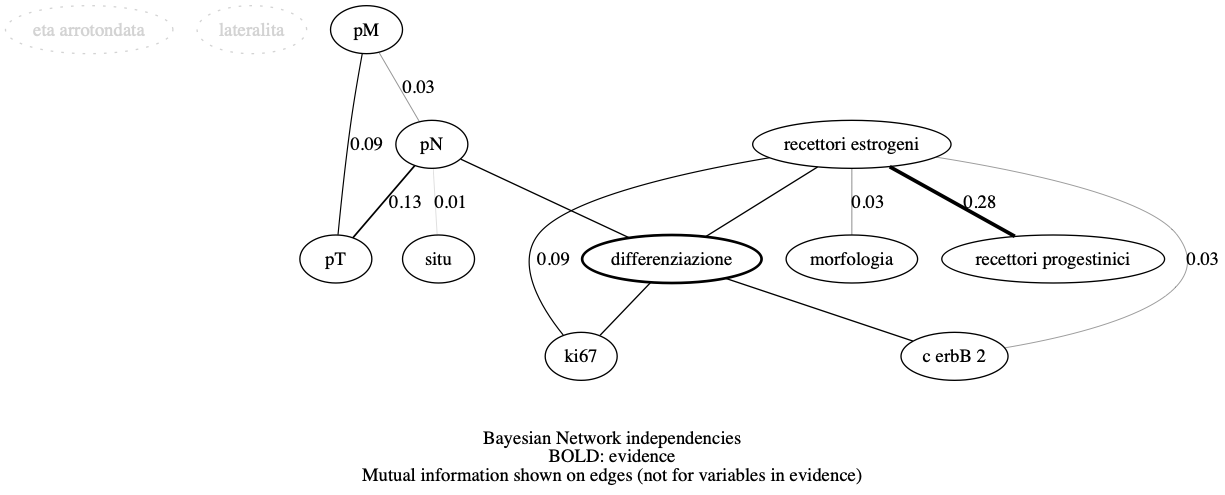
\includegraphics[width=\columnwidth]{methodology/images/example-d-separation-mpe_1}}
\caption{Example output during the first round of the d-separation-aware variant of \texttt{dialogue}.
	The variable \enquote{mut17q21} is the initial evidence.}
\label{fig:pseudo-mpe-independencies_1}
\end{figure}

\begin{figure}[htbp]
\centerline{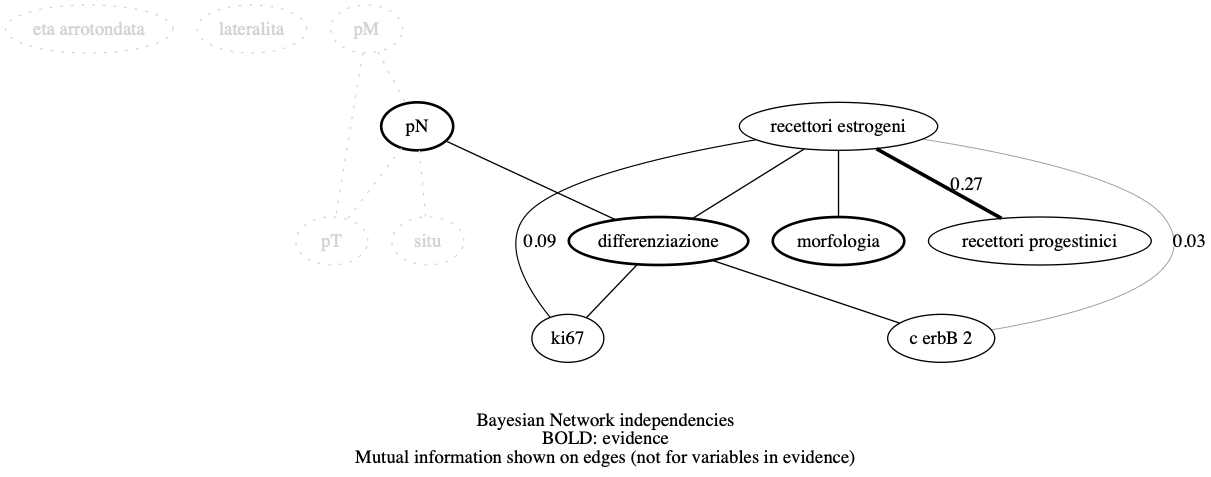
\includegraphics[width=\columnwidth]{methodology/images/example-d-separation-mpe_2}}
\caption{Example output during the second round of the d-separation-aware variant of \texttt{dialogue}.
	\enquote{morfologia} is added to the evidence set and this makes a large part of the network redundant.}
\label{fig:pseudo-mpe-independencies_2}
\end{figure}

\todo{implementare e finire}
\begin{algorithm}[htp!]
	\caption{Thresholded pseudo-MPE algorithm}
	\label{alg:pseudo-mpe-thresholded}
	\begin{algorithmic}
		\STATE $separated\_list = \emptyset$
		\STATE {\bf input:} source $X$, evidence $E$, nodes $V$
		\FOR{target $Y \in V$} 
		\STATE append $d-separated(X, Y, E)$ to $separated\_list$ \COMMENT{will return true or false}
		\ENDFOR
		\STATE {\bf output:} $separated\_list$
	\end{algorithmic}
\end{algorithm} 

\subsubsection{Alternative Explanation Branches}
The function to generate alternative branches to the main MPE branch in the dialogue tree is called after the user refuses a $(state,value)$ in the dialogue and accepts one of the the alternatives.
The motivation is to present the user with a simple \enquote{what-if} analysis, replying to the question \enquote{Had I accepted the $(state,value)$ presented me by the system, what would have been the most probable configuration of the remaining $(state,value)$ pairs?}.
The question is answered by generating a maximally probable, alternative MPE sub-branch rooted in the last node in the main MPE branch that is under construction through the dialogue.

The alternative branch is generated by what is essentially an automated version of \texttt{dialogue} that always accepts the first suggestion returned by \texttt{next\_most\_probable\_states}.
Given that \texttt{dialogue} and \texttt{generate\_alternative\_branch} are essentially one and the same, the latter inherits the same pruning strategies as the former.
That is, \texttt{generate\_alternative\_branch} called during the exhaustive dialogue will generate a maximally likely assignment over all variables in $V \smallsetminus E$ while when invoked from one of the other two variant of the dialogue algorithm, it will apply their same pruning strategies.

The implementation of the MPE Tree was based on the \texttt{Anytree} python package (see Subsec. \ref{subsec:libraries}).
This lightweight package lacks in flexibility but makes the creation of a tree very simple.
Creation of a new node is done by simply passing a pointer to the parent node to the \texttt{Node} object constructor.
Construction of trees composed of chains, as are the ones I am dealing with, can be done by simply keeping track of the pointer to the last inserted node.

An example of the output shown to the user at each step of the dialogue is shown in Fig. \ref{fig:alternative-branch_1} while the pseudocode for the three variants are shown in Alg. \ref{alg:alternative-branch-echaustive}, \ref{alg:alternative-branch-independencies} and \ref{alg:alternative-branch-thresholded}.
Note that $alternative\_evidence$ is local to this algorithm and is separate from the $evidence$ used in the main \texttt{dialogue} procedure.

\begin{figure}[htbp]
\centerline{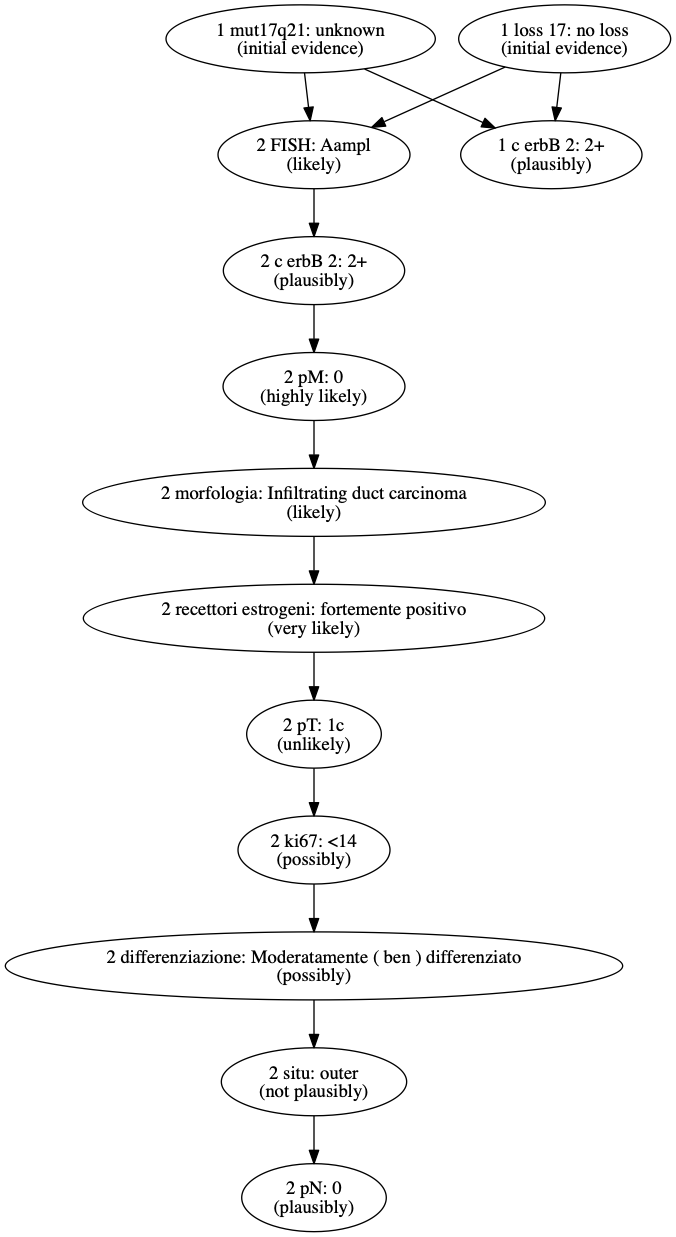
\includegraphics[width=\columnwidth]{methodology/images/alternative-explanation-tree-example}}
\caption{Example output at the end of the d-separation-aware variant of \texttt{dialogue}.
	The tuple (\enquote{ki67},\enquote{<14}) was proposed but the expert refused it and accepted the alternative (\enquote{c erbB 2},\enquote{0}).
	The main MPE Branch has ID 1 while the \enquote{what-if} one has ID 2.}
\label{fig:alternative-branch}
\end{figure}

\begin{algorithm}[htp!]
	\caption{Exhaustive alternative explanation branch algorithm}
	\label{alg:alternative-branch-echaustive}
	\begin{algorithmic}
		\STATE $alternative\_evidence = evidence$ 
		\STATE $alt\_node = $ last node in the main MPE Tree
		\STATE $branch\_id = branch\_id + 1$
		\WHILE{True} 
			\STATE $mpe\_states$ = \texttt{next\_most\_probable\_states($alternative\_evidence$)}
			\IF{$mpe\_states$ is empty}
				\STATE return
			\ELSE
				\STATE $next\_state$ = head of $mpe\_states$ 
				\STATE create $next\_state$ node, tag it with $branch\_id$ and make it son of $alt\_node$
				\STATE update $alt\_node$ node to be $next\_state$ node
				\STATE $alternative\_evidence = alternative\_evidence \cup next\_state$
			\ENDIF
		\ENDWHILE
	\end{algorithmic}
\end{algorithm}

\begin{algorithm}[htp!]
	\caption{Independencies alternative explanation branch algorithm}
	\label{alg:alternative-branch-independencies}
	\begin{algorithmic}
		\STATE $alternative\_evidence = evidence$ 
		\STATE $alt\_node = $ last node in the main MPE Tree
		\STATE $branch\_id = branch\_id + 1$
		\WHILE{True} 
			\STATE $separated = $ \texttt{evidence\_d\_separation($alternative\_evidence$)}
			\STATE $mpe\_states$ = \texttt{next\_most\_probable\_states($alternative\_evidence$)}
			\STATE $mpe\_states = mpe\_states \smallsetminus separated$ 
			\IF{$mpe\_states$ is empty}
				\STATE return
			\ELSE
				\STATE $next\_state$ = head of $mpe\_states$ 
				\STATE create $next\_state$ node, tag it with $branch\_id$ and make it son of $alt\_node$
				\STATE update $alt\_node$ node to be $next\_state$ node
				\STATE $alternative\_evidence = alternative\_evidence \cup next\_state$
			\ENDIF
		\ENDWHILE
	\end{algorithmic}
\end{algorithm} 

\todo{implementare e fare}
\begin{algorithm}[htp!]
	\caption{Independencies alternative explanation branch algorithm}
	\label{alg:alternative-branch-thresholded}
	\begin{algorithmic}
		\STATE $evidence = $ user selected $(state,value)$ tuples
		\STATE $MPE\_tree = $ root MPE Tree in $evidence$
		\WHILE{True} 
			\STATE $separated = $ \texttt{evidence\_d\_separation()} \COMMENT{based on evidence of previous step}
			\STATE $mpe\_states$ = \texttt{next\_most\_probable\_states()}
			\STATE $mpe\_states = mpe\_states \smallsetminus separated$ 
			\IF{$mpe\_states$ is not empty}
				\STATE $next\_state$ = head of $mpe\_states$ 
				\STATE propose $next\_state$ to user \COMMENT{the least entropic state}
				\IF{the user refuses $next\_state$}
					\FOR{$alternative\_state$ in $mpe\_states \smallsetminus next\_state$}
						\STATE propose $alternative\_state$ to user \COMMENT{the next least entropic states}
						\IF{the user accepts $alternative\_state$}
							\STATE call \texttt{generate\_alternative\_branch()} on $MPE\_tree$ 
							\STATE add $alternative\_state$ to $MPE\_tree$
							\STATE $evidence = evidence \cup alternative\_state$
						\ELSE
							\STATE continue \COMMENT{go to next proposal}
						\ENDIF
					\ENDFOR
				\ELSE
					\STATE add $next\_state$ to $MPE\_tree$
					\STATE $evidence = evidence \cup next\_state$
				\ENDIF
			\ELSE 
				\STATE return 
			\ENDIF
		\ENDWHILE
	\end{algorithmic}
\end{algorithm} 

\todo{ancora da implementare true MPE}
\subsubsection{\enquote{Pseudo-MPE} from Random Evidence} \label{subsubsec: pseudo-mpe-random}
In order to compare the Pseudo-MPE output with the true MPE solution I implemented a simple algorithm that, starting from a random initial set of evidence, generates the relative pseudo-MPE and MPE solutions.
The random initial evidence set is constructed by randomly choosing a number in the interval $k = [ 1, |V| ]$, with $V$ the set of vertices in the BN, and then randomly selecting $k$ of the random variables in $V$ to yield the set of variables $E$.
The value of each variable is randomly chosen among the set of its values; as all variables are categorical, this can easily be done.

\todo{vedere perchè magari sposto tutta l'implementazione su MPE\_Graph quando metto evidenze multiple ovunque}
The implementation is based on the \texttt{NetworkX} python library (see Subsec. \ref{subsec:libraries}) package as what is being constructed is not a tree but a \textit{polytree} (see Subsec. \ref{subsec:graph-theory}), as nodes may have multiple parents.
\texttt{NetworkX} is a much more complete package that \texttt{Anytree} and this allows greater flexibility, at the cost of slightly more complexity.
Note that $alternative\_evidence$ is considered separate from the main $evidence$ used in \texttt{dialogue}.

The pseudocode is shown in Alg. \ref{alg:pseudo-mpe-random-evidence} while an example output can be seen in Fig. \ref{fig:pseudo-mpe-random}.

\begin{algorithm}[htp!]
	\caption{Pseudo-MPE from random evidence algorithm}
	\label{alg:pseudo-mpe-random-evidence}
	\begin{algorithmic}
		\STATE $evidence = \emptyset$
		\STATE generate random number $k \in [ 1, |V| ]$
		\STATE $S = $ choose $k$ variables from $V$
		\FOR{$s \in S$}
			\STATE choose random $v$ in the possible values of $e$ 
			\STATE $evidence = evidence \cup (s,v)$
		\ENDFOR
		\STATE $MPE\_tree = $ MPE Tree rooted in $evidence$
		\STATE $last\_node = evidence$
		\STATE $alternative\_evidence = evidence$ 
		\WHILE{True} 
			\STATE $mpe\_states$ = \texttt{next\_most\_probable\_states($alternative\_evidence$)}
			\IF{$mpe\_states$ is empty}
				\STATE return
			\ELSE
				\STATE $next\_state$ = head of $mpe\_states$ 
				\STATE create $next\_state$ node and make it son of $last\_node$
				\STATE update $alt\_node$ node to be $next\_state$ node
				\STATE $alternative\_evidence = alternative\_evidence \cup next\_state$
			\ENDIF
		\ENDWHILE
	\end{algorithmic}
\end{algorithm}

\begin{figure}[htbp]
\centerline{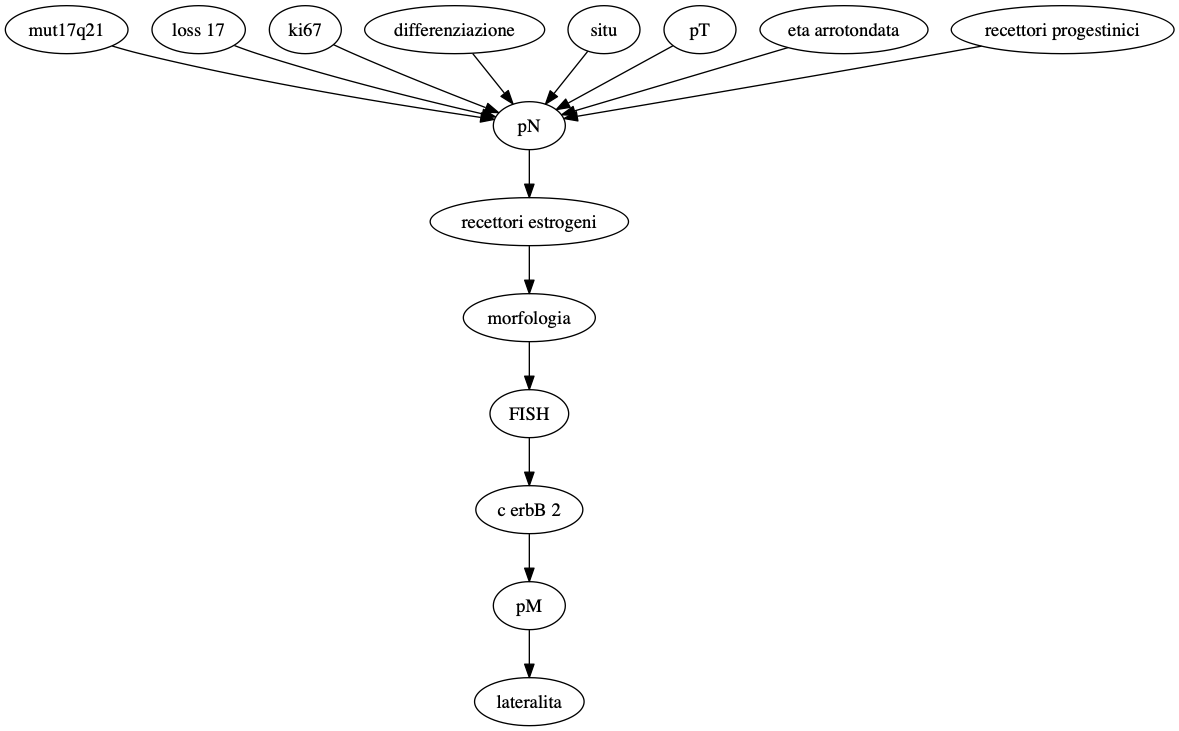
\includegraphics[width=\columnwidth]{methodology/images/pseudo-mpe-random-example}}
\caption{Example output of the Pseudo-MPE from random evidence algorithm.}
\label{fig:pseudo-mpe-random}
\end{figure}

\subsubsection{Inverse Explanation}
\todo{da fare e trovare nome migliore}

\subsubsection{Natural Language Explanation}
\todo{da fare e magari pensare anche a visual explanations?}
The probability of each proposed tuple is quantified in natural language based on the probability of the most probable value within the variable.
These are shown in Tab. \ref{tab:naturallanguageprobabilities}.

\begin{table*}[htbp]
\caption{Probability quantifiers in natural language}
\begin{tabularx}{\textwidth}{@{} X X @{}}
\toprule 
Probability range & Natural language quantifier \\
\midrule 
(0, 0.2) &  "highly unlikely" \\
(0.2, 0.3) & "very unlikely" \\
(0.3, 0.4) & "unlikely" \\
(0.4, 0.5) & "not plausibly" \\
(0.5, 0.6) & "plausibly" \\
(0.6, 0.7) & "possibly" \\
(0.7, 0.8) & "likely" \\
(0.8, 0.9) & "very likely" \\
(0.9, 1) &  "highly likely" \\
(1) &  "certain" \\
\bottomrule
\end{tabularx}
\label{tab:naturallanguageprobabilities}
\end{table*}


\subsubsection{Pairwise Correlations} \todo{per ora non funziona}
An interesting addition is an algorithm to measure the interrelatedness between pairs of variables.

